% !Mode:: "TeX:UTF-8"

\chapter{实验过程与结果分析}
\label{experiment}
本章将介绍本项目的实验部分,包括对KITTI数据集、数据预处理、模型训练以及实验结果分析等内容。在结果分析中,我们首先比较DODT各模块对结果的影响,以考察每个模块的有效性;然后我们探讨了关键帧的选取步长对三维物体检测结果的影响,以便确定最优的步长;最后我们也测试了DODT在多目标追踪任务上的性能,并与前沿方法对比。结果显示DODT框架能很好的完成流数据的三维物体检测以及多目标跟踪任务。

\section{KITTI数据集介绍}
\label{kitti}
本项目的所有实验都是基于无人驾驶领域中广泛使用的KITTI公开数据集开展的。KITTI数据集是由德国卡尔斯鲁厄理工学院和丰田美国技术研究院联合采集的,该数据集包含多种传感器数据:一个惯性导航系统(GPS/IMU,型号为OXTS RT 3003)数据,一个激光雷达(Velodyne HDL-64E)数据,两个灰度相机数据(140万像素)以及两个彩色相机数据(140万像素)。其中激光雷达扫描频率为10帧/秒,相机基本与地平面保持平行,图像采集的尺寸为$1382 \times 512$像素。所有传感器的整体布局如\figurename \ref{fig:KITTI}。

\begin{figure}[h]
	\centering
	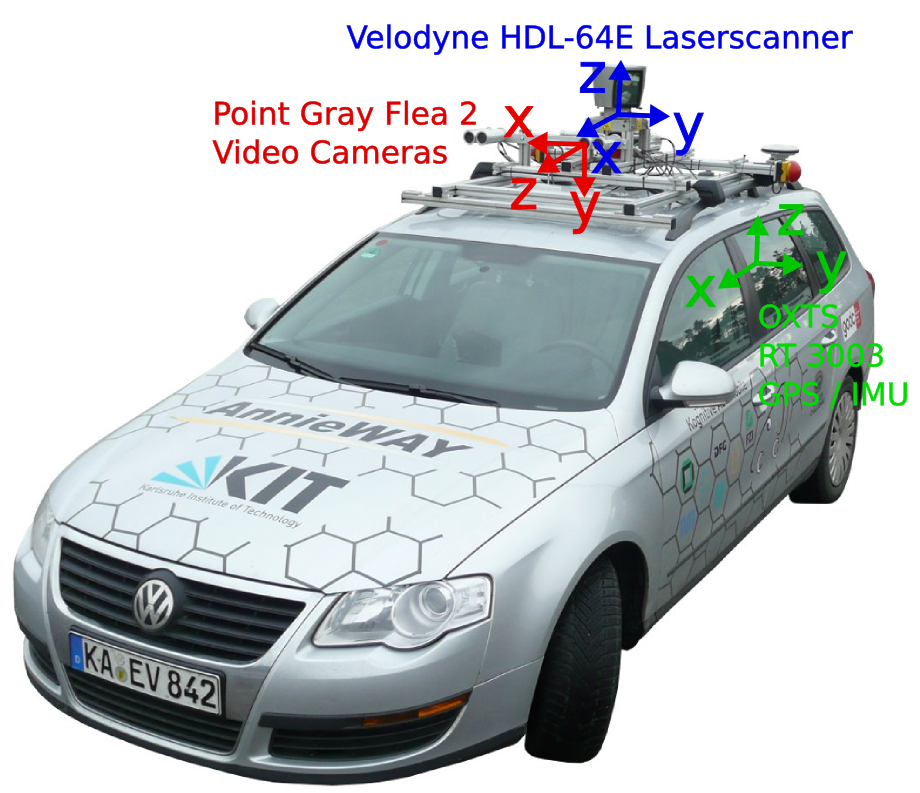
\includegraphics[width=0.6\textwidth]{./imgs/KITTI.png}
	\caption{KITTI数据集传感器整体布局。}
	\label{fig:KITTI}
\end{figure}

KITTI数据集根据不同的任务分为stero、flow、scenceflow、depth、odometry、object以及tracking等部分,对应着场景流估计、深度估计、路径规划、物体检测以及目标追踪等任务。每一个任务数据包都包含了海量的训练数据以及测试数据,供研究者使用。本项目主要使用了KITTI数据集的tracking数据包,该数据包由21段训练视频流(共8004帧数据)以及29段测试视频流(共11095帧数据)组成。每一段视频流都是由连续的RGB图像帧以及三维点云帧组成,在训练数据集中,还包含了每一帧数据对应的二维目标框(针对图像数据)以及三维目标框(针对点云数据)。此外,针对每一段视频流,KITTI还提供了传感器的标定信息以及每一帧的GPS/IMU数据,供研究者数据标定时使用。

多目标追踪的标签共有10项,记录了帧的信息以及帧中每个目标的信息。信息列举如下:
\begin{itemize}
	\item frame id:帧的编号;
	\item object id:每一帧中目标的编号,也是轨迹的编号;
	\item type:目标的类别,有”Car“,”Van“, "Trunk",”Pedestrian“,”Cyclist“等类别,本实验将”Car“和”Van“合并为”Car“类,并只针对”Car“类进行检测和追踪;
	\item truncated:标记目标是否被图像边界截断,”0“表示不截断,”1“表示截断;
	\item occluded:标记目标被遮挡的程度,共有0到3四个取值,”0“表示完全可视,”1“表示部分遮挡,”2“表示大部分遮挡,”3“表示完全遮挡;
	\item alpha:目标的观测角,$\alpha \in [-\pi, \pi]$;
	\item bbox:物体在图像上的2D边界框,包含左上角,右下角的坐标值;
	\item dimensions:物体的高、框和长,单位为米;
	\item location:物体底部中心点在相机坐标系的三维坐标 x,y,z,单位为米;
	\item ry:物体在相机坐标系沿Y轴的旋转角,$r_y \in [-pi, pi]$。
\end{itemize}
其中目标的观测角$\alpha = -[(\pi+r_y) + (\pi+\beta)]$,$r_y$与$\beta$如\figurename \ref{fig:kitti_obj}所示,而目标的location坐标如\figurename \ref{fig:kitti_box3d}所示。
\begin{figure}[!t]
	\centering
	\begin{minipage}[t]{0.5\textwidth}
		\centering
		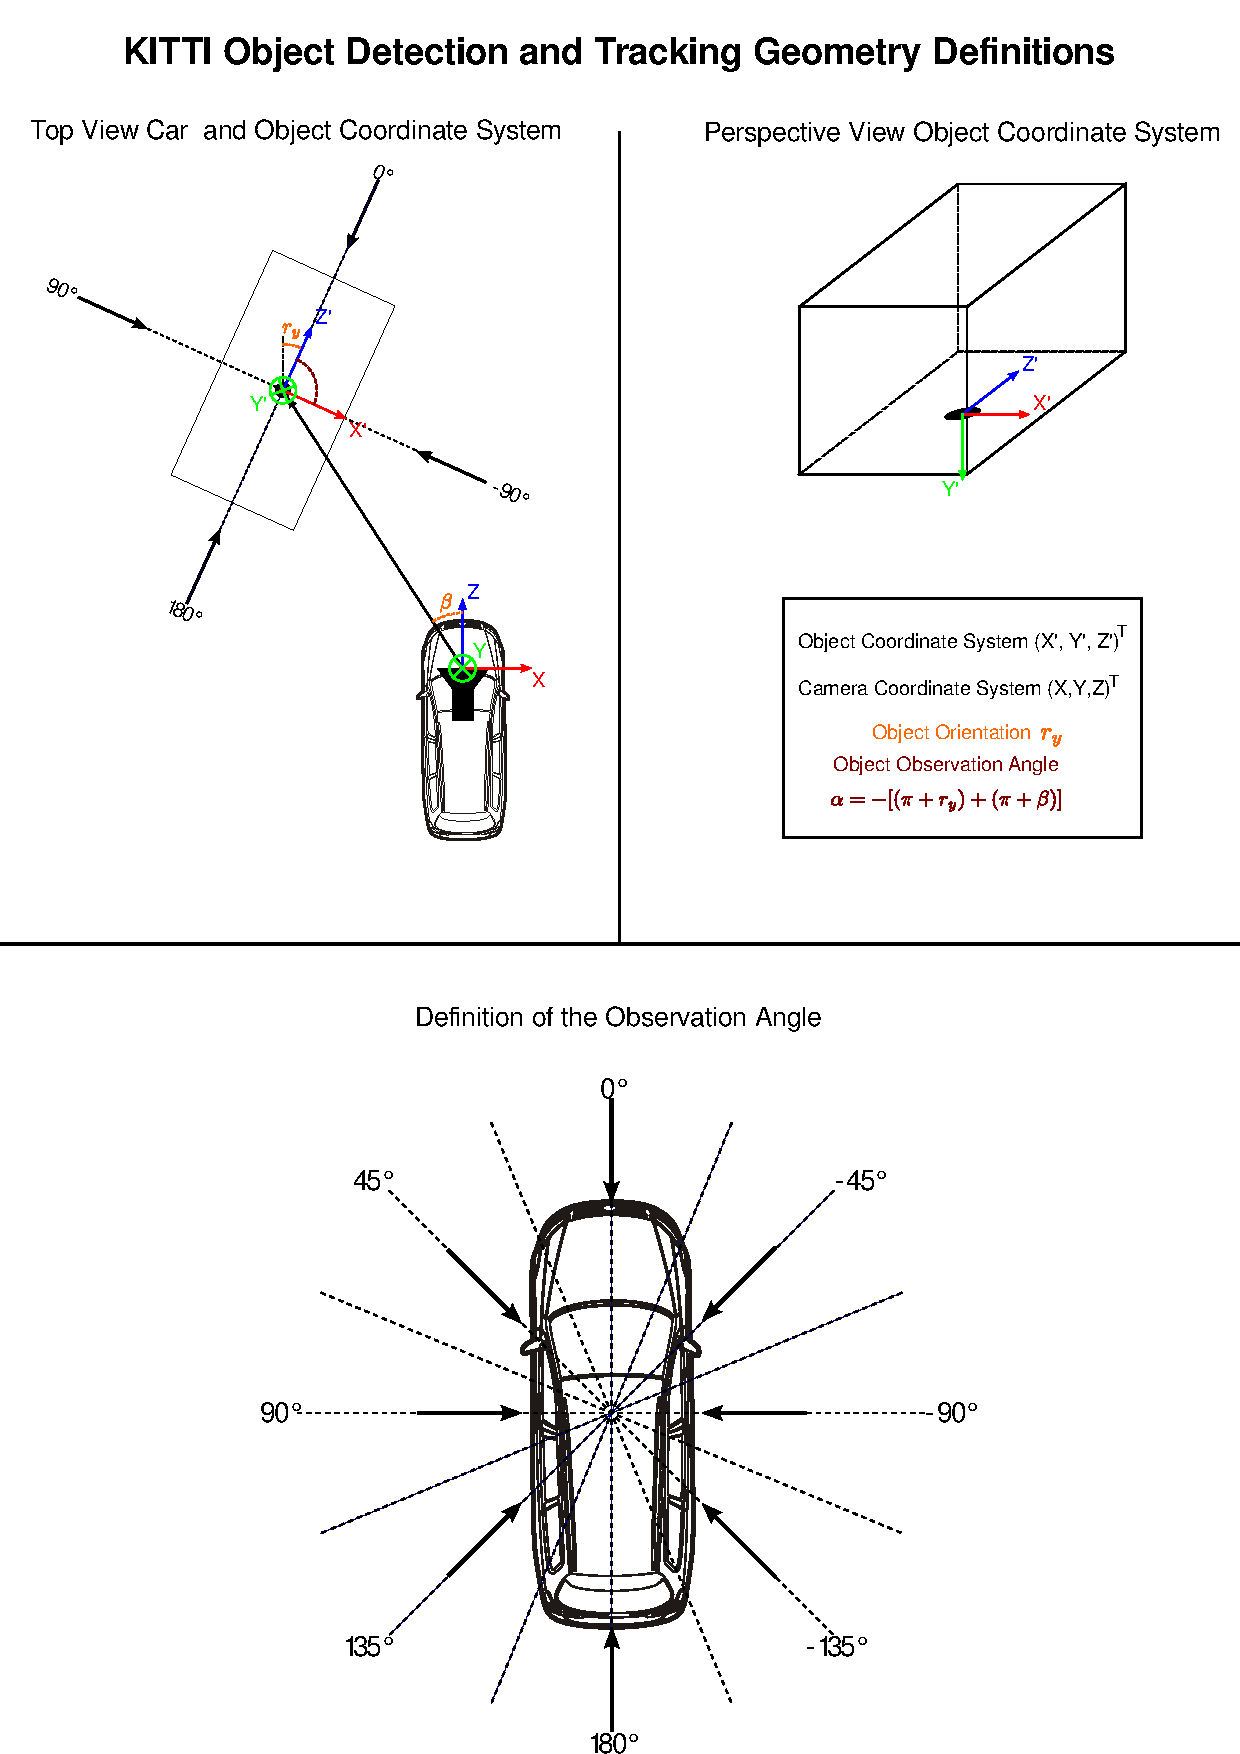
\includegraphics[trim={0cm, 15cm, 12cm, 2.5cm}, clip,width=\textwidth]{./imgs/KITTI_obj.pdf}
		\caption{KITTI数据集观测角与转向角示意图。}
		\label{fig:kitti_obj}
	\end{minipage}
	\begin{minipage}[t]{0.48\textwidth}
		\centering
		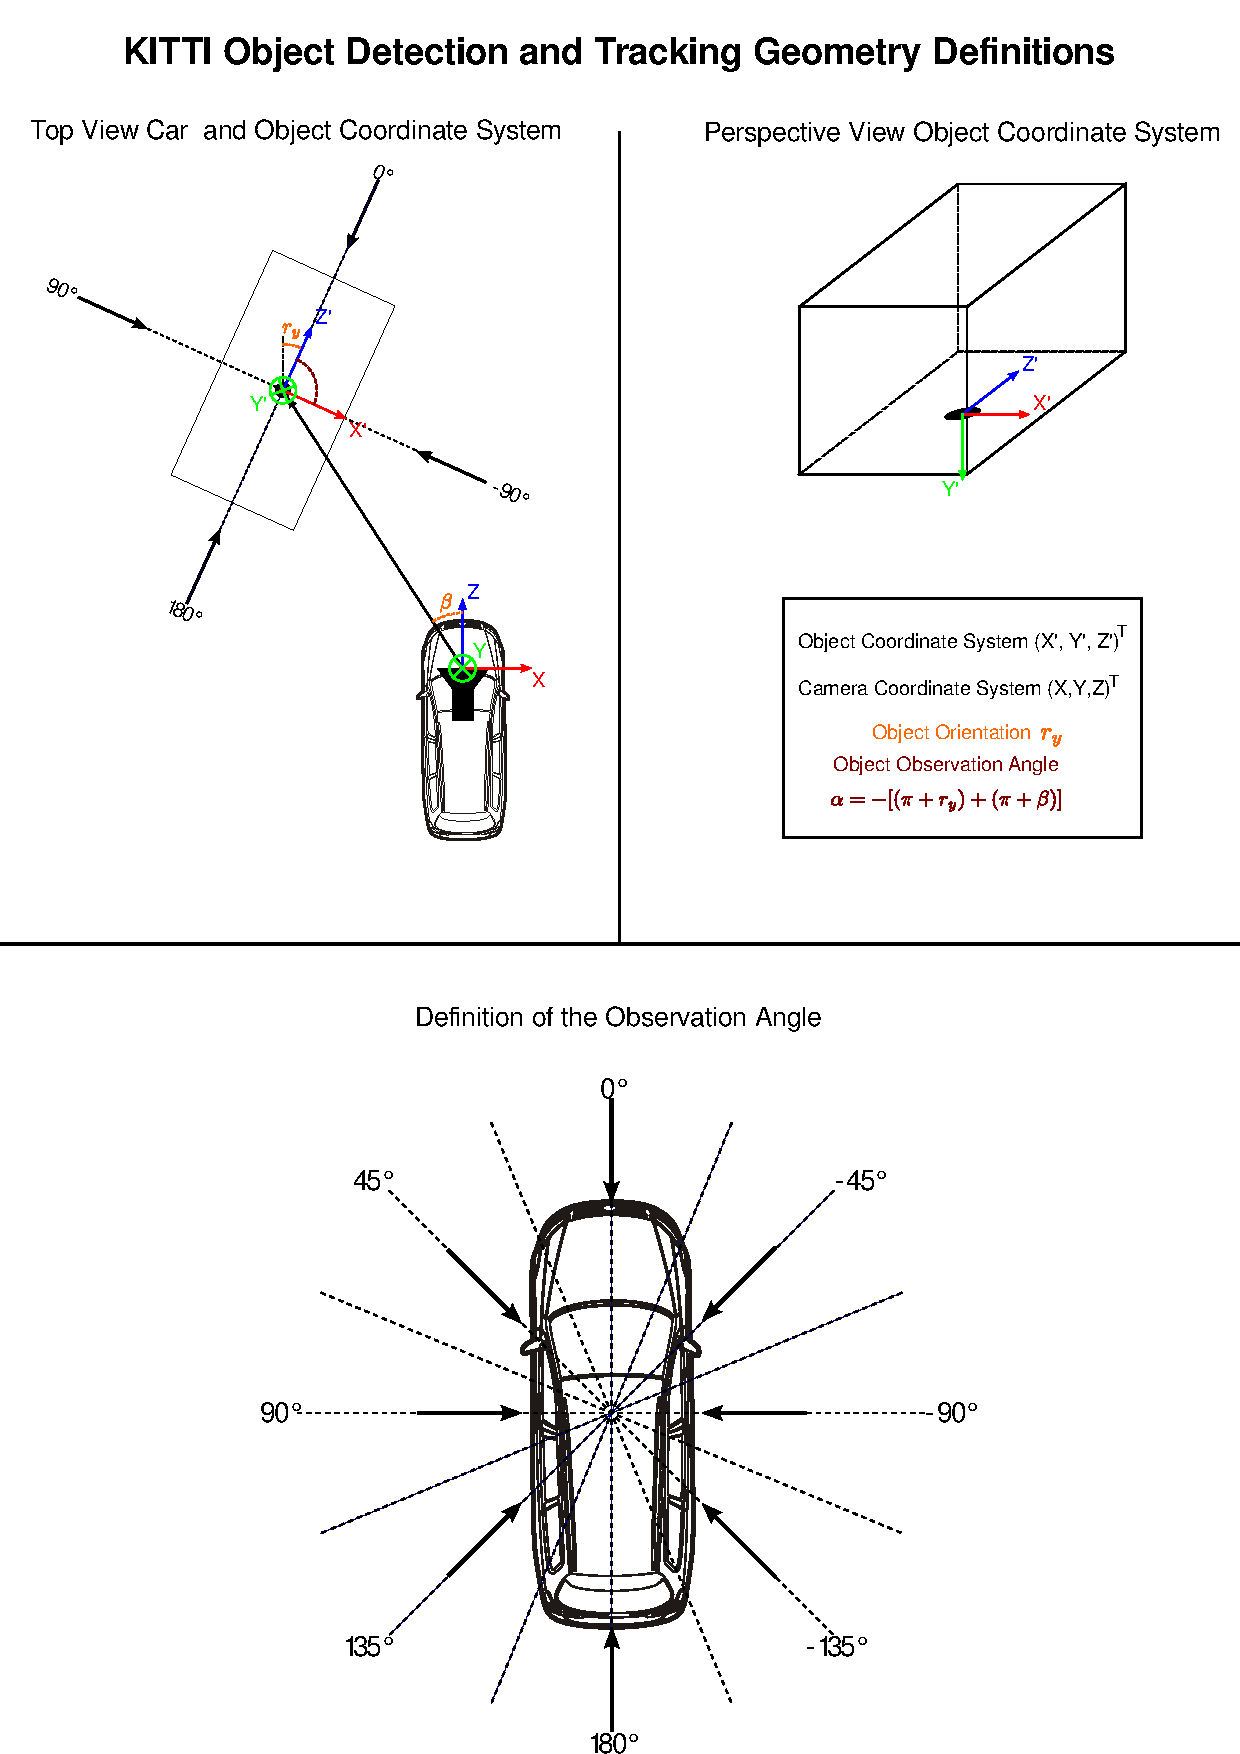
\includegraphics[trim={12cm, 20cm, 1.8cm, 2.5cm}, clip,width=\textwidth]{./imgs/KITTI_obj.pdf}
		\caption{KITTI数据集目标的位置坐标。}
		\label{fig:kitti_box3d}
	\end{minipage}
\end{figure}


传感器的标定信息保存在”calib.txt“文件中,其中包含了相机的参数矩阵以及各传感器之间的旋转矩阵。信息列举如下:
\begin{itemize}
	\item P0-P3:四个相机的内参矩阵 $P \in \mathcal{R}^{3\times 4}$;
	\item R0\_rect:$\mathcal{R}^{3\times 3}$,将摄像机坐标系转换到图像坐标系的校准矩阵;
	\item Tr\_velo\_to\_cam:$\mathcal{R}^{3\times 4}$,激光雷达坐标系到摄像机坐标系的旋转矩阵;
	\item Tr\_imu\_to\_velo:$\mathcal{R}^{3\times 4}$,IMU坐标系到激光雷达坐标系的旋转矩阵。
\end{itemize}

GPS/IMU数据提供了30项信息,其中包含每一帧中自身车辆的经纬度、海拔、三个欧拉角(roll,yaw以及pitch)、速度、加速度、角速度等信息。本实验主要使用到了经纬度以及欧拉角信息将不同帧之间的信息校准到同一坐标系。欧拉角包含了偏航角(yaw,表示机体轴在水平面上的投影与地轴之间的夹角,右偏为正)、俯仰角(pitch,表示机体轴与地平面之间的夹角,抬头为正) 以及翻滚角(roll,表示机体对称面绕机轴转动的角度,右滚为正),如\figurename \ref{fig:euler}所示。

\begin{figure}[t]
	\centering
	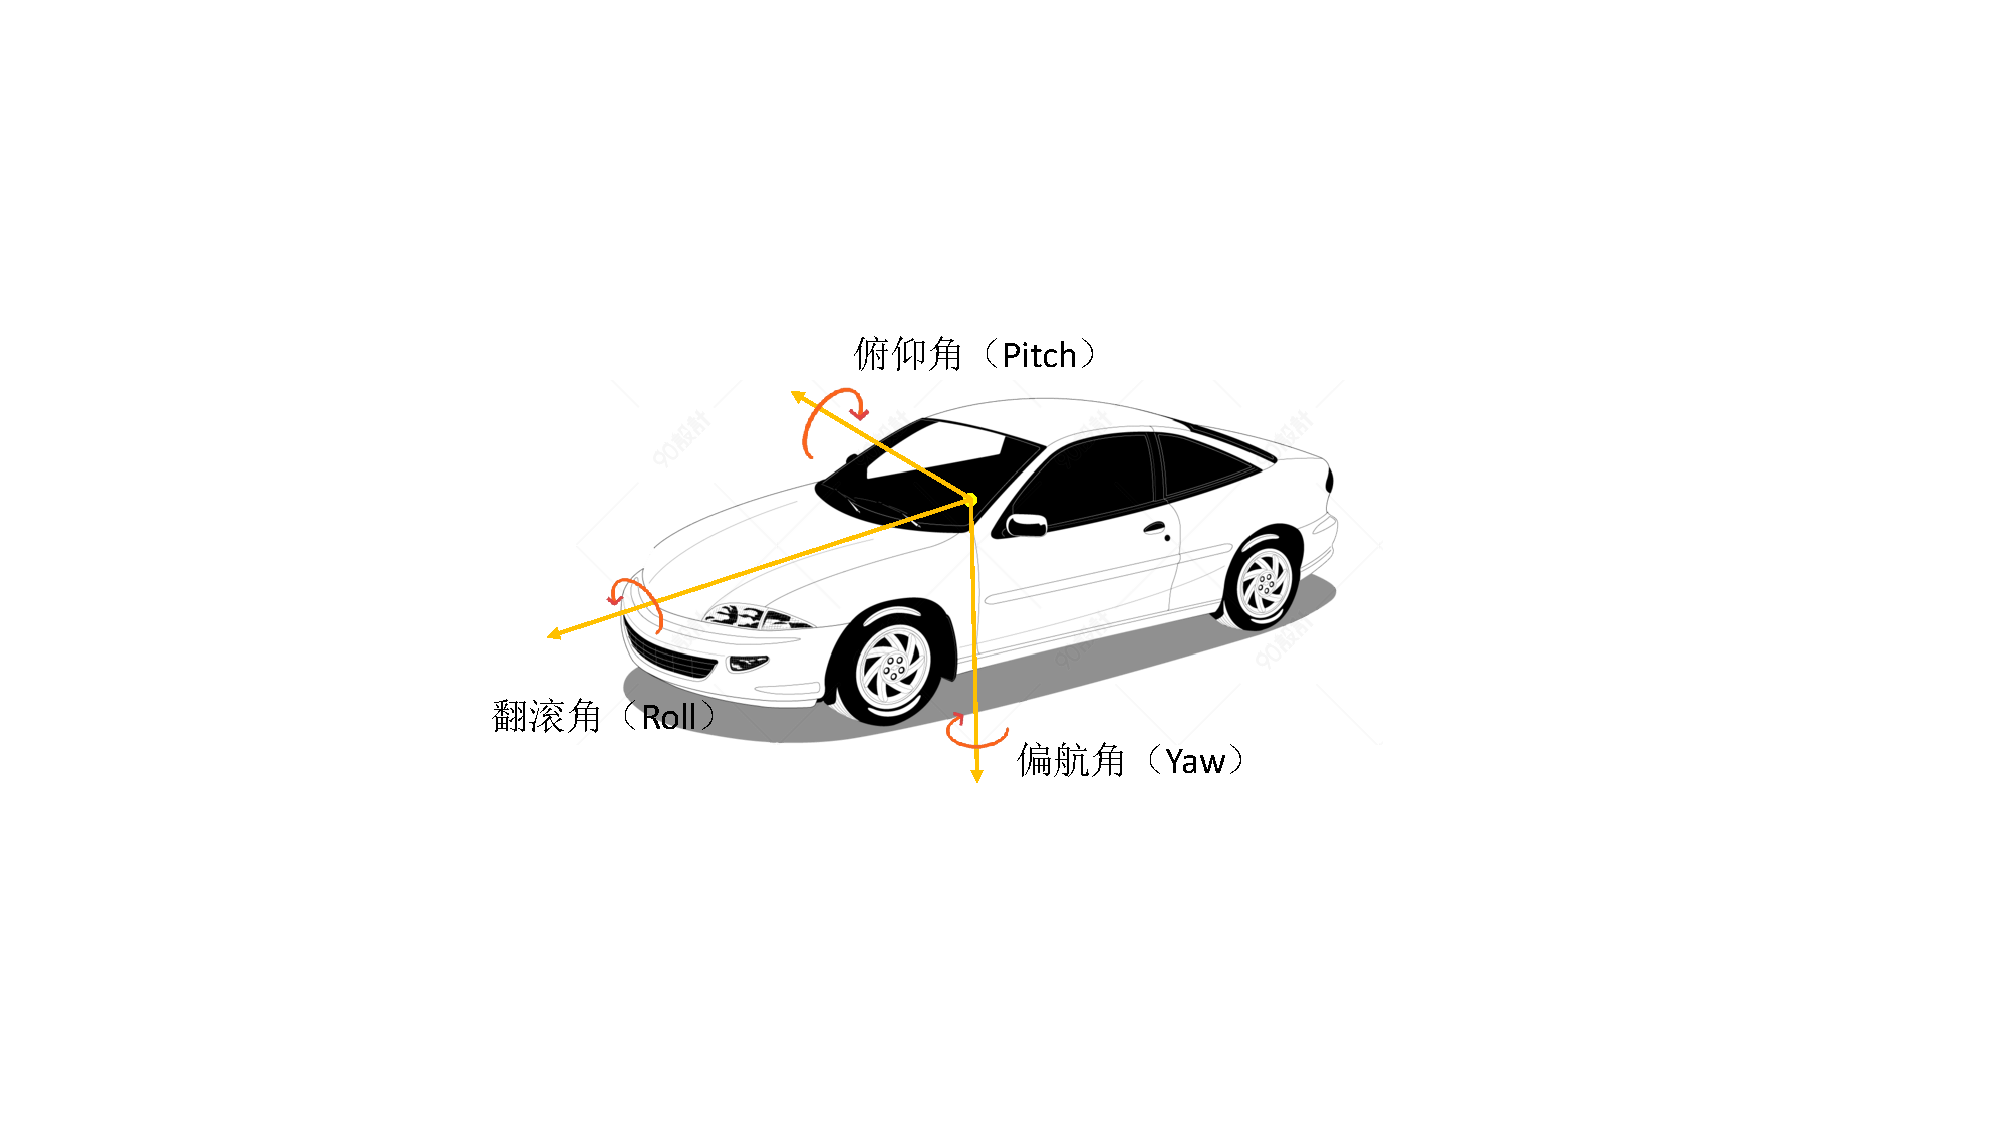
\includegraphics[trim={5cm, 6cm, 5cm, 5cm}, clip,width=\textwidth]{./imgs/euler.pdf}
	\caption{三个欧拉角的方向示意图。}
	\label{fig:euler}
\end{figure}



\section{数据预处理}
\label{preprocessing}
DODT框架融合了点云数据信息以及RGB图像数据信息,由于激光雷达的视野和摄像机的视野不同,因此在融合之前需要将激光雷达坐标系下的点云转换到图像坐标系中。假设激光雷达坐标系下点云的齐次坐标为$P_{pc}=[X,Y,Z,1]^T$,其中$X=(x_1,x_2,...,x_n),Y=(y_1,y_2,...,y_n),Z=(z_1,z_2,...,z_n)$,表示点云中所有$n$个点的坐标向量。点云中所有点对应到图像坐标系上的像素点齐次坐标为$P_{img} = [U,V,1]^T$(U,V同样为坐标向量),则转换关系如公式\ref{con:transform}所示。其中$P_{cam}$为相机的参数矩阵,R0\_rect 以及 Tr\_velo\_to\_cam为上一小节校准文件中的转换矩阵。
\begin{equation}
P_{img} = P_{cam} * R0\_rect * Tr\_velo\_to\_cam * P_{pc}
\label{con:transform}
\end{equation}
经过这步转换后,点云与图像都在相同坐标系下。之后我们对点云的预处理方式和AVOD\cite{ku2018joint}一样,首先将落在图像尺寸之外的点过滤掉,然后分别沿X,Z,Y轴截取$[-40,40] \times [0,70] \times [0,2.5]$米的区域作为最终的点云数据。

为了让DODT输入的两帧关键帧数据能够很好的融合从而得到时序信息,我们还需要将两帧数据校准到同一坐标系,该过程需要用到上文提及的GPS/IMU数据。假设DODT输入的相邻关键帧为$F_1$和$F_2$,$F_1$对应时刻车体的经纬度为 $(lat_1, lon_1)$,欧拉角pitch、roll、yaw 为 $(p_1,r_1,y_1)$,$F_2$ 对应时刻车体的经纬度为 $(lat_2, lon_2)$,欧拉角pitch、roll、yaw为 $(p_2,r_2,y_2)$。则$F_1$和$F_2$坐标系原点的球面距离计算公式如\ref{con:sphere_dis}所示,其中$R=6378137.0$米,为地球的半径。
\begin{equation}
d = 2R * \arcsin(\sqrt{\sin^2(\frac{lat_2 - lat_1}{2}) + \cos(lon_1)\cos(lon_2)\sin^2(\frac{lon_2 - lon_1}{2})})
\label{con:sphere_dis}
\end{equation}
为了将$F_2$的点云数据转换到$F_1$坐标系下,需要求得两坐标系的位移$\Delta$以及旋转矩阵$\mathcal{M}$。根据计算的两坐标原点的球面距离以及各自的欧拉角,位移$\Delta$计算如公式\ref{con:origin_offset}所示,旋转矩阵$\mathcal{M} = R_Z * R_X * R_Y$,计算如公式\ref{con:rotate_matrix}所示,其中$\delta_p = (p_2 - p_1)$,$\delta_r = (r_2 - r_1)$,$\delta_y = (y_2 - y_1)$,为两帧车体欧拉角的偏差。 假设$F_2$中所有点云的原始坐标矩阵为$P_{origin} = [X,Y,Z]^T \in \mathbb{R}^{ n \times 3}$,则其转换到$F_1$坐标系下的坐标矩阵$P_{trans} = (P_{origin} + \Delta) * \mathcal{M}$。坐标系转换前后两帧点云数据叠加可视化对比如下图所示,由图可知坐标系转换有利于两帧信息的关联。 
\begin{equation}
\Delta = [\delta_x, \delta_y, \delta_z]^T = [d\cos(y_2-y_1), d\sin(y_2-y_1),d\sin(p_2-p_1)]
\label{con:origin_offset}
\end{equation}
\begin{equation}
\mathcal{M} = \\
	\begin{bmatrix} 
		\cos(\delta_p) & 0 & \sin(\delta_p)\\
		0 & 1 & 0 \\
		-\sin(\delta_p) & 0 & \cos(\delta_p)
	\end{bmatrix}
	\begin{bmatrix} 
	1 & 0 & 0\\
	0 & \cos(\delta_r) & -sin(\delta_r) \\
	0 & sin(\delta_r) & \cos(\delta_r)
	\end{bmatrix}
	\begin{bmatrix} 
	\cos(\delta_y) & -\sin(\delta_y) & 0\\
	\sin(\delta_y) & \cos(\delta_y) & 0 \\
	0 & 0 & 1
	\end{bmatrix}
\label{con:rotate_matrix}
\end{equation}

在数据可视化时,我们注意到KITTI官方提供的多目标追踪标签并不完备。例如,在图\ref{fig:examples}第一行中,我们可视化了训练数据集第0段视频的几帧数据以及官方提供的标签,可以看到有些目标(由红色虚线框圈出)在128帧中有标签,但是在118以及120帧中却没有标签,尽管这些目标在118帧以及120帧中都能很好识别。这种情况在整个训练数据集中都经常出现,因此,为了更好的衡量DODT模型的检测与追踪性能,我们手动添加了这些漏打的标签。

\section{模型训练}
\label{training}
我们的实验在一台配置有Telsa P100 的GPU以及Intel(R) Xeon(R) E5-2667 v4 @ 3.20GHz的32核CPU的服务器上进行。为了训练并验证DODT的性能,我们将KITTI提供的21段训练视频流分成两份,视频编号为奇数为训练集,偶数的为验证集。我们将官方标记的”Car“以及”Van“目标都当做”Car“,只做该类别的检测与追踪。网络训练过程中的大部分超参数设置我们都借鉴了AVOD\cite{ku2018joint}。具体而言,DODT在训练数据集中迭代次数为120K,批处理大小为1。DODT使用ADAM\cite{kingma2014adam}作为优化器,并且使用了初始值为0.0001,每迭代30K步以0.8的因子指数下降的可变学习率。网络的损失值由四部分组成,目标检测的分类和回归损失以及时序信息模块的分类与回归损失,如公式\ref{con:total_loss}所示。其中训练时权重$w_{cls}, w_{reg}, w_{co}, w_{corr}$的值分别为1.0,5.0,1.0,1.0。RPN的参数设置以及NMS算法的阈值设置在第三章方法部分有详细介绍,这里不再赘述。
\begin{equation}
L_{total} = w_{cls}L_{cls} + w_{reg}L_{reg} + w_{co}L_{co} + w_{corr}L_{corr}
\label{con:total_loss}
\end{equation}

\section{实验结果分析}
\label{results}

在实验阶段,我们首先测试了\textit{Shared RPN}模块对候选框预测的性能提升,然后使用控制变量法分析了DODT各模块对最终检测结果的影响,这些模块包括\textit{Shared RPN}模块、时序信息处理模块以及运动插值模块。接着我们探究了不同关键帧选取步长对流数据三维物体检测的性能影响,最后我们探究了不同模块对DODT在多目标追踪任务上性能的影响。

\subsection{三维物体检测结果分析}
\label{ablation_study}
\begin{table}[t]
	\centering
	\wuhao
	\caption{候选框预测性能比较。}
	\vspace{0.3cm}
	\begin{tabular}{ccc}
		\toprule[1.5pt]
		方法        & 原始 RPN & \textit{Shared RPN}  \\ \midrule
		准确率(\%)  & 97.81      & \textbf{98.47}       \\
		\bottomrule[1.5pt]
	\end{tabular}
	\label{table:rpn_result}
\end{table}

RPN在目标检测任务中用于候选框的提取,为了衡量\textit{Shared RPN}相对于原始RPN的性能提升,我们比较了两者预测候选框的准确率,结果如表\ref{table:rpn_result}所示。
由表格可知,原始的RPN模块(直接使用AVOD\cite{ku2018joint}中的RPN)对候选框的预测准确率为97.81\%,而\textit{Shared RPN}的预测准确率为98.47\%,比前者提升了0.66\%。这说明\textit{Shared RPN}使用多帧数据能够生成更为准确的候选框。此外,由于\textit{Shared RPN}在不引入额外计算量的情况下一次性可生成供两帧使用的候选框,因此其运行帧率是原始RPN的两倍。

\begin{table}\centering
	\wuhao
	\caption{DODT的不同设置在验证数据集上的结果(只预测“Car”类别)。每项的指标为$AP_{3D}/AP_{BEV}$ (\%), 为三维物体检测在3D视角和BEV视角的平均精度。 “S” 表示\textit{Shared RPN}模块, “T” 表示时序信息处理模块, “M” 表示运动插值模块。 $\tau$ 是关键帧选取步长。} 
	\vspace{0.3cm}
	\resizebox{\textwidth}{!}{
		\begin{tabular}{ccccccccc}
			\toprule[1.5pt]
			&\multicolumn{1}{c|}{}   & \multicolumn{3}{c|}{IoU = 0.5}  		         & \multicolumn{3}{c|}{IoU = 0.7}          &  \\ \midrule
			\multicolumn{1}{c|}{方法} & \multicolumn{1}{c|}{模块}    & Easy     & Moderate   & \multicolumn{1}{c|}{Hard}     & Easy  & Moderate & \multicolumn{1}{c|}{Hard}    & FPS \\\midrule
			\multicolumn{1}{c|}{AVOD\cite{ku2018joint}}     &\multicolumn{1}{c|}{-}     & 90.13 / 90.91  & 80.00 / 81.79 & \multicolumn{1}{c|}{71.61 / 81.79}  & 76.00 / 90.90 & 57.23 / 81.73 & \multicolumn{1}{c|}{56.13 / 72.69}   & 10.0\\
			\multicolumn{1}{c|}{DODT($\tau$ = 1)}     &\multicolumn{1}{c|}{S}     & 88.28 / 99.97  & 85.74 / 90.90 & \multicolumn{1}{c|}{86.14 / 90.89}  & 83.44 / 90.82 & 67.48 / 90.79 & \multicolumn{1}{c|}{61.24 / 90.80}     & 6.7 \\
			\multicolumn{1}{c|}{DODT($\tau$ = 1)}     &\multicolumn{1}{c|}{S+T}     & 88.32 / \textbf{99.99}  & 86.53 / 90.90 & \multicolumn{1}{c|}{86.71 / \textbf{90.90}}  & 83.60 / 90.82 & 68.93 / 90.80 & \multicolumn{1}{c|}{62.69 / 90.81}   & 5.9\\
			\multicolumn{1}{c|}{DODT($\tau$ = 1)}     &\multicolumn{1}{c|}{S+M}     & 89.99 / 99.95  & 87.86 / 90.87 & \multicolumn{1}{c|}{87.81 / 90.86}  & 86.89 / 90.89 & 73.96 / 90.83 & \multicolumn{1}{c|}{67.07 / 81.79}   & 6.5\\
			\multicolumn{1}{c|}{DODT($\tau$ = 1)}     &\multicolumn{1}{c|}{S+T+M} & \textbf{90.63} / 99.95  & 89.07 / 90.90 & \multicolumn{1}{c|}{88.79 / \textbf{90.90}}  & 88.74 / 90.91 & 75.27 / 90.84 & \multicolumn{1}{c|}{68.75 / 90.57}   & 5.7\\ \midrule
			\multicolumn{1}{c|}{DODT($\tau$ = 2)}     &\multicolumn{1}{c|}{S+T+M} & 90.60 / 99.94  & \textbf{89.19 / 90.91} & \multicolumn{1}{c|}{\textbf{88.91} / 90.88}  & \textbf{88.90 / 90.92} & \textbf{76.64} / 90.85 & \multicolumn{1}{c|}{75.81 / 90.83}   & 8.6\\
			\multicolumn{1}{c|}{DODT($\tau$ = 3)}     &\multicolumn{1}{c|}{S+T+M} & 90.61 / 99.98  & 89.01 / 90.89 & \multicolumn{1}{c|}{88.84 / 90.89}  & 88.81 / 90.91 & 76.38 / \textbf{90.86} & \multicolumn{1}{c|}{\textbf{75.83 / 90.85}}   & 11.4\\
			\multicolumn{1}{c|}{DODT($\tau$ = 4)}     &\multicolumn{1}{c|}{S+T+M} & 90.55 / 99.94  & 88.82 / 90.88 & \multicolumn{1}{c|}{88.34 / 90.87}  & 88.43 / 90.91 & 75.70 / 90.82 & \multicolumn{1}{c|}{68.75 / 90.82}   & 14.3\\
			\multicolumn{1}{c|}{DODT($\tau$ = 5)}     &\multicolumn{1}{c|}{S+T+M} & 87.98 / 90.91  & 85.57 / 90.87 & \multicolumn{1}{c|}{86.01 / 90.87}  & 81.59 / 90.81 & 67.30 / 90.76 & \multicolumn{1}{c|}{61.35 / 81.73}   & 17.1\\
			\multicolumn{1}{c|}{DODT($\tau$ = 6)}     &\multicolumn{1}{c|}{S+T+M} & 78.77 / 90.75  & 70.88 / 90.71 & \multicolumn{1}{c|}{71.65 / 81.70}  & 71.71 / 90.44 & 55.86 / 81.50 & \multicolumn{1}{c|}{56.80 / 81.51}   & \textbf{20.0} \\ 
			\bottomrule[1.5pt]
	\end{tabular}}
	\label{table:result_detection}
\end{table}



为了验证各模块对DODT三维物体检测任务性能的影响,我们进行了消融实验,实验结果如表\ref{table:result_detection} 上半部分所示,$\tau = 1$表示输入的两关键帧为相邻帧。目标检测的评价指标为平均精度(Average Precision,AP),即计算检测正确的目标个数占总目标个数的百分比,然后对目标种类做平均。衡量物体检测是否正确需要计算预测框与真实框的IOU,若IOU大于某一阈值则判断为检测正确。本实验统计了两种不同阈值的实验结果,分别为0.5和0.7。此外,KITTI根据目标遮挡情况的不同将检测任务分为”Easy”、“Moderate”和“Hard”三类,其中”Easy”对应无遮挡目标(occluded = 0)的检测结果,“Moderate”对应部分遮挡(occluded = 1) 目标的检测结果,而“Hard”则对应大部分遮挡(occluded = 2) 目标的检测结果。

\textit{Shared RPN}的对比结果对应与表格第一行与第二行,在使用其他新模块的基础上,使用原始RPN模块的DODT相当于AVOD架构,因此我们直接对比了AVOD和只使用了\textit{Shared RPN}模块的DODT($\tau = 1$)的是实验结果。由结果可知,\textit{Shared RPN}模块基本在所有指标上都能带来检测性能的提升。特别的,对于IOU = 0.7的阈值下,\textit{Shared RPN}在”Easy”、“Moderate”和“Hard”检测级别上分别为$AP_{3D}$带来了7.44\%、10.26\%和5.11\%的性能提升。这些显著的性能提升要归功于\textit{Shared RPN}模块能够结合多帧信息预测更为精确的候选框。另外,从结果可知使用\textit{Shared RPN}可以显著提高检测速度,这主要是相邻两帧复用了候选框,节省了不少时间。

在基础DODT框架(双路结构 + \textit{Shared RPN})的基础上,我们加入了时序信息处理模块(T),实验结果如表\ref{table:result_detection}第三行所示。对比第二行的基础DODT框架结果,在IOU=0.7的阈值下,时序信息处理模块在”Easy”、“Moderate”和“Hard”检测级别上分别为$AP_{3D}$带来了0.16\%、1.45\%和1.45\%的性能提升。结果显示时序信息模块能够提升遮挡目标的检测性能,这是因为时序模块能够融合两帧关键帧的信息,目标在某一帧被遮挡的话很有可能在下一帧不被遮挡。由于在BEV视角上目标遮挡很少,且候选框层次的特征融合让两关键帧信息可以互补,使得DODT对于困难样本的预测更加准确。

为探究运动插值模块对DODT目标检测性能的影响,我们在基础DDOT框架的基础上加入了运动插值模块(M),实验结果如表\ref{table:result_detection}第四行所示。结果显示在IOU=0.5的阈值下,运动插值模块在”Easy”、“Moderate”和“Hard”检测级别上分别为$AP_{3D}$带来了1.71\%、2.12\%和1.67\%的性能提升;而在IOU=0.7的阈值下则分别带来了3.45\%、6.48\%和5.83\%的性能提升。这些结果表明运动插值模块能够显著提高DODT对车辆的检测性能,特别是对于困难目标的检测。对比不同IOU阈值的结果还可以看出,运动插值模块能够显著改善预测框偏离真实框较大的情况。这些提升显示了我们的MoI算法能够根据前后帧的检测结果筛除检测错误的样本,并且能够通过轨迹的历史状态进一步延伸轨迹。此外,时序信息处理模块和运动插值模块联合使用的话能够额外提升1~2\%的性能,如表格\ref{table:result_detection}第五行所示。这是因为运动插值模块在时序信息处理模块输出结果的基础上能够运行的更好,详情可参阅第三章3.5小节中MoI算法的介绍。

\begin{figure}[!t]
	\centering
	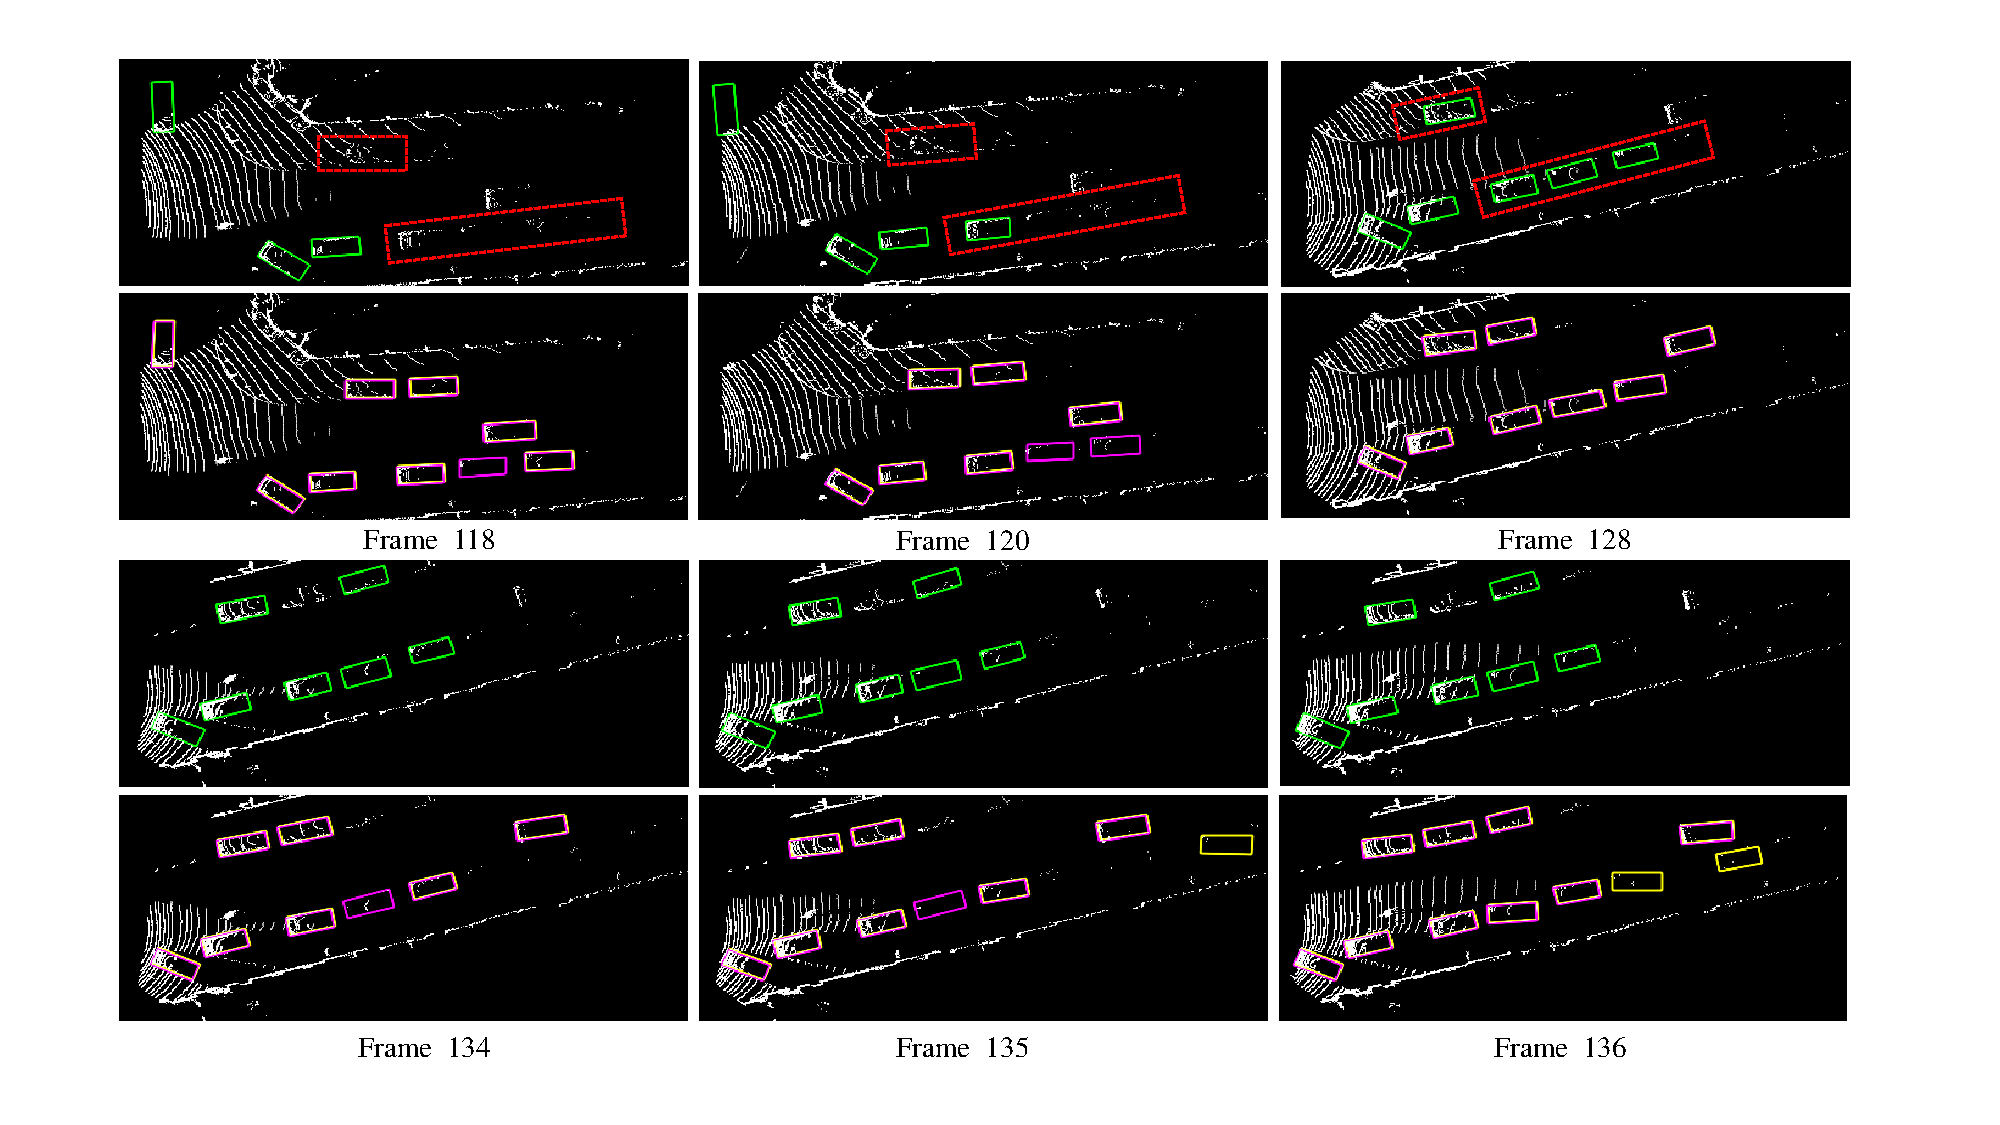
\includegraphics[trim={2cm, 1cm, 2.5cm, 1cm}, clip, width=\textwidth]{./imgs/examples.pdf}
	\vspace{-1.0cm}
	\caption{视频序列0的标签以及预测结果可视化。\textcolor{green}{绿色}为官方提供的标签框, \textcolor{yellow}{黄色}是时序步长$\tau = 1$的预测结果,\textcolor{magenta}{洋红色}为时序步长$\tau = 3$的预测结果。混合颜色的框是黄色框和洋红色框重叠造成的,该结果最好彩色打印查看。}
	\label{fig:examples}
\end{figure}


\subsection{流数据物体检测结果分析}
\label{stream_result}

%\begin{figure}[!t]
	\centering
	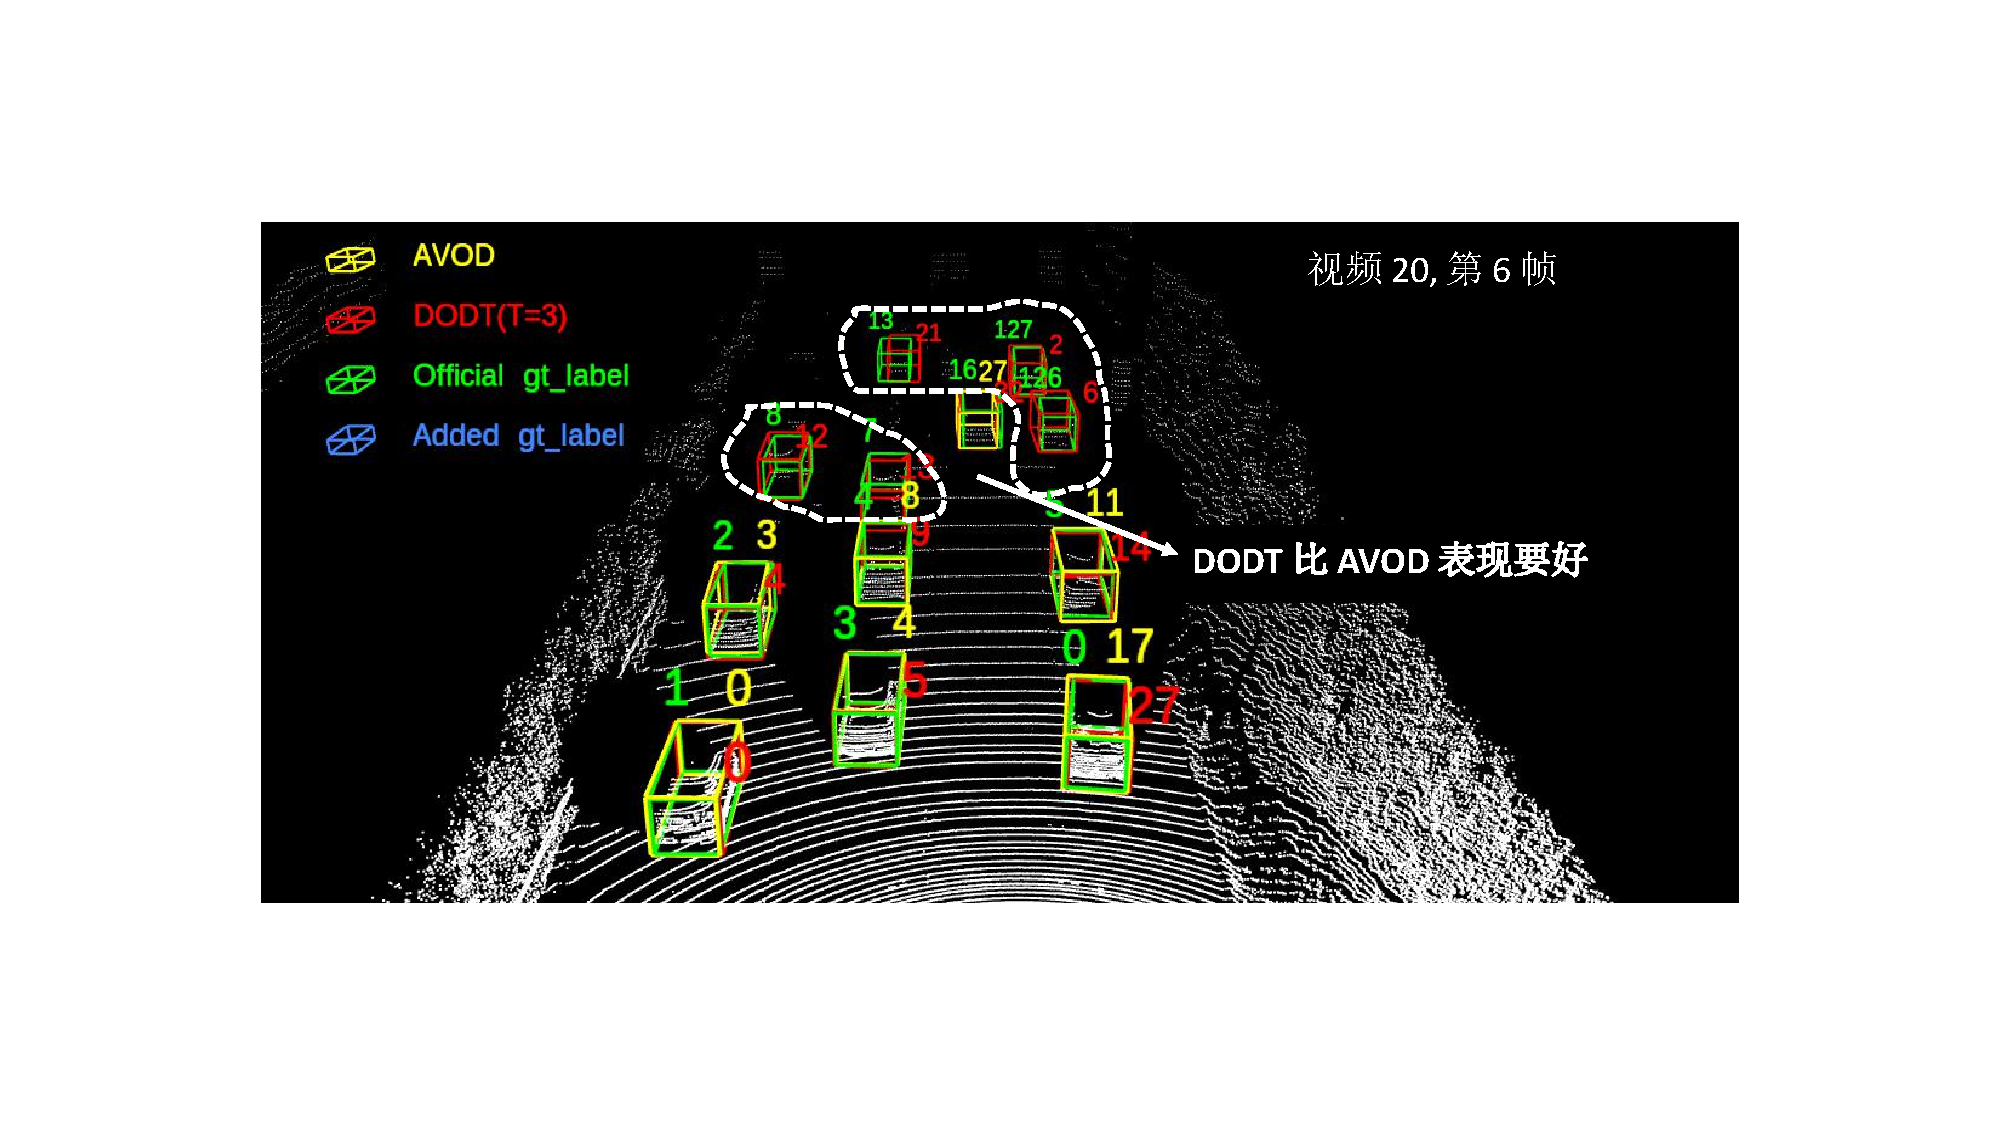
\includegraphics[trim={4cm, 4cm, 5cm, 3.7cm}, clip, width=\textwidth]{./imgs/result_compare_01.pdf}
	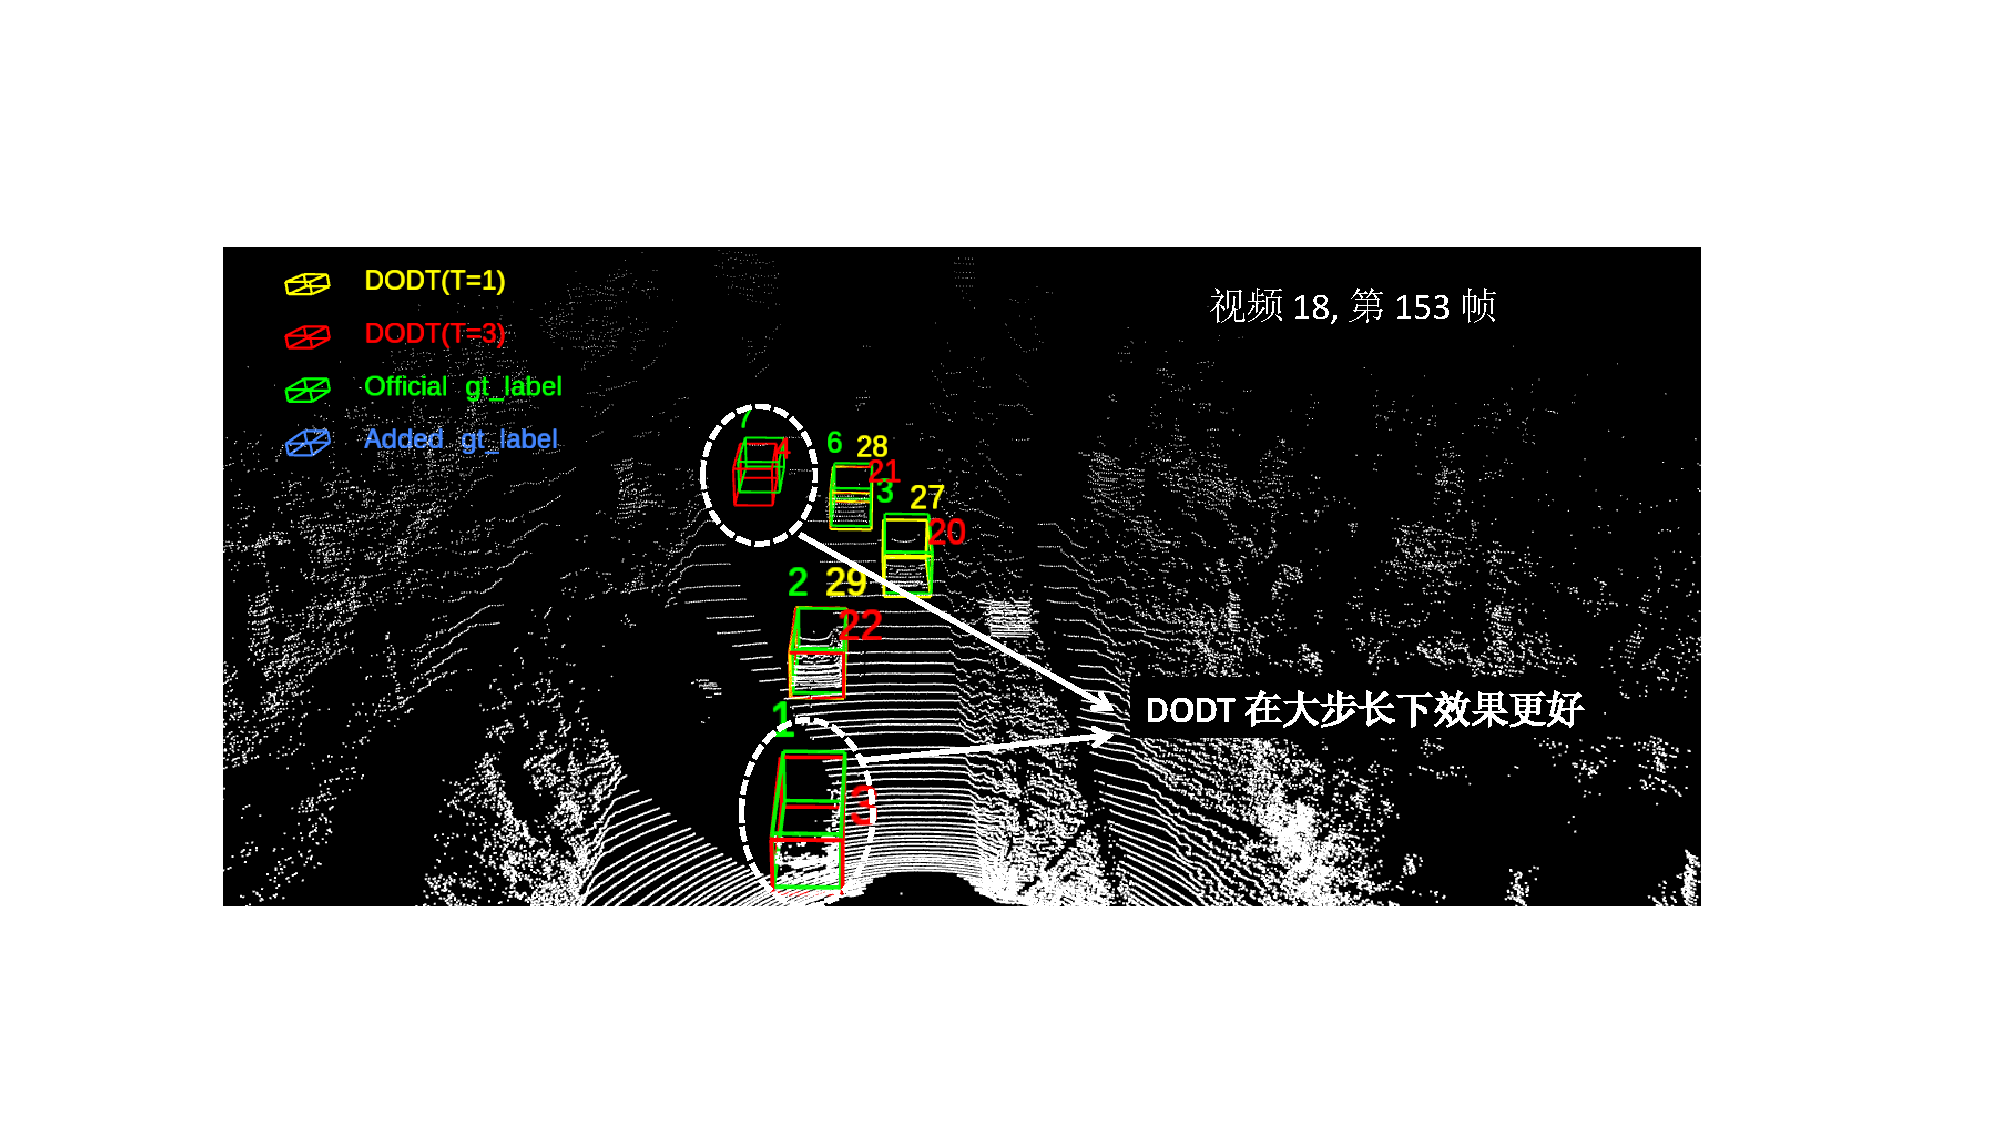
\includegraphics[trim={4cm, 4cm, 5cm, 3.7cm}, clip, width=\textwidth]{./imgs/result_compare_02.pdf}
	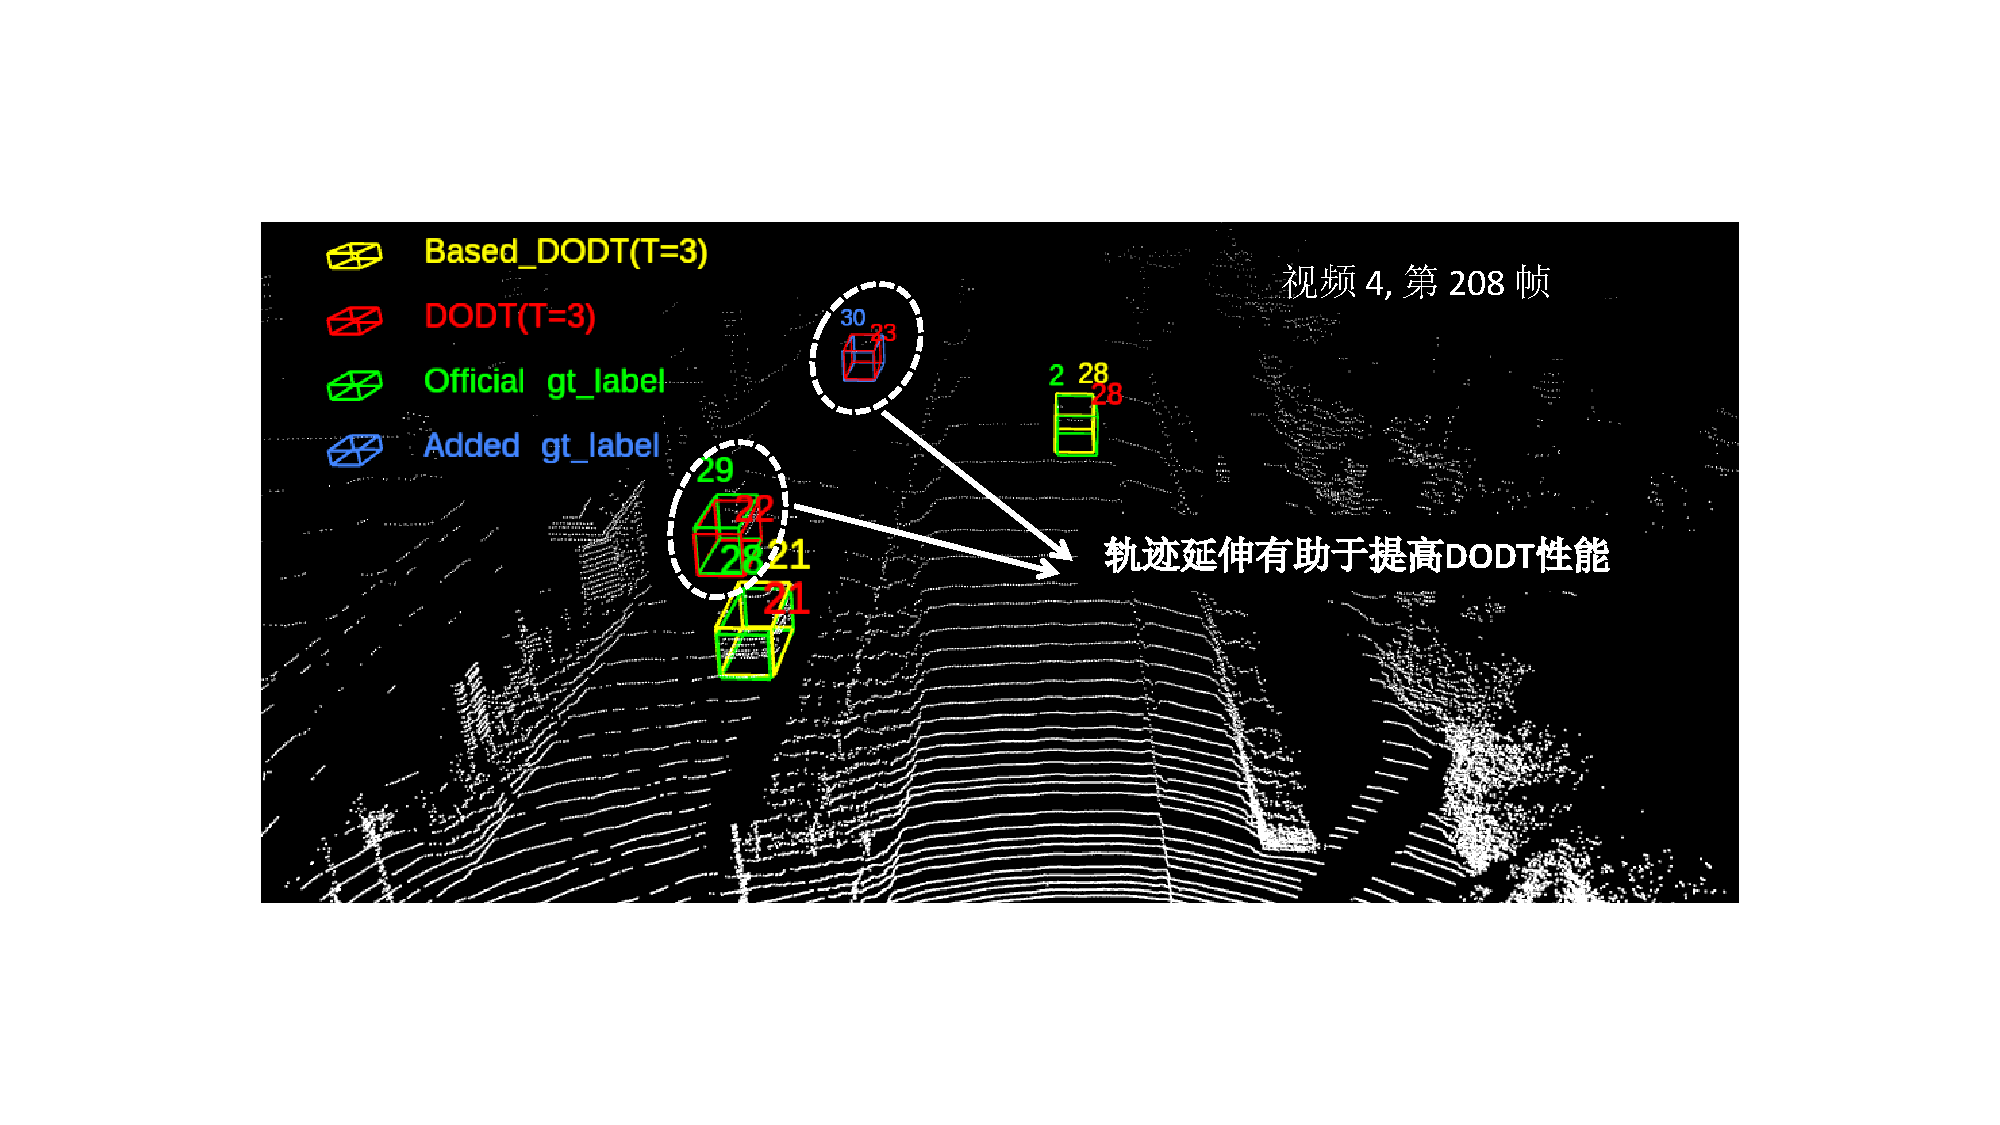
\includegraphics[trim={4cm, 4cm, 5cm, 3.5cm}, clip, width=\textwidth]{./imgs/result_compare_03.pdf}
	\caption{不同模型结果对比可视化。第一幅图的结果显示DODT在远处要比AVOD表现的好,第二幅图的结果显示DODT在大步长下要比小步长性能好,第三幅图的结果显示使用MoI算法进行轨迹延伸的效果要更好。最好查看彩色版本。}
	\label{fig:result_compare}
\end{figure}


DODT框架同时处理两帧相邻的关键帧,非关键帧的检测结果是通过关键帧结果插值得到,因此关键帧的选取对于流数据物体检测影响很大。由于在三维空间中,车辆是连续运动,因此不存在像图像数据中的突变现象,每一帧都可作为关键帧使用。但是输入两帧关键帧的时间跨度对DODT的检测性能影响很大,如果步长太小,则会造成检测速度慢,时序信息处理变得很累赘;如果步长太大,则两帧关键帧数据信息关联度不高,时序信息提取困难。为了探索最佳的关键帧选取步长$\tau$,我们一系列对比实验。在完整版DODT框架(\textit{Shared RPN} + 时序信息处理模块 + 运动插值模块)框架的基础上,通过改变步长$\tau$的值($\tau \in \{1,2,3,4,5,6\}$),我们得到了六组不同的实验结果,如表\ref{table:result_detection}下半部分所示。从结果可以看出,IOU=0.7的阈值下,DODT($\tau = 2$)在”Easy”和“Moderate”检测级别上表现最佳,分别为88.90\%和76.64\%($AP_{3D}$)。而DODT($\tau = 3$)在“Hard”检测级别上表现最佳,为75.84\%($AP_{3D}$),并且在”Easy”和“Moderate”检测级别上也与$\tau = 2$时有相当的性能。对比于DODT($\tau = 1$),当$\tau = \{2,3\}$时DODT在困难样本上的检测性能显著提升,“Moderate”任务上提升约1\%而“Hard”任务提升有约7\%。这说明当选取一个较大的步长时,DODT对遮挡目标的检测能力显著提高。这些提升很大程度上是由MoI算法带来的,我们可视化了几帧数据,如图\ref{fig:examples}下半部分所示。其中洋红色的预测框为DODT($\tau=3$)的预测结果,黄色框为$\tau = 1$的预测结果。可以看出,较大的步长能够筛除错误的检测结果,并且也能够更好的补全轨迹两端缺失的目标。

然而并不是步长$\tau$越大检测结果越好,从表\ref{table:result_detection}可以看出,当$\tau = \{4,5,6\}$时,DODT的检测性能下降很快。这一方面是因为长距离的时序信息更难捕捉,另一方面是因为大步长不利于MoI算法对非关键帧的插值以及轨迹的延伸。当步长太长时,两关键帧之间有很多非关键帧,目标的跳跃较大,不利于插值算法的运行。我们也计算了不同步长时DODT的运行帧率,结果如表\ref{table:result_detection}最后一列所示。DODT两三维目标检测分支的总运行时间为175ms/帧(Telsa P100 GPU),当步长$\tau$增大时,检测分支以及时序信息处理模块的运行时间保持不变,而插值算法的运行时间增加可忽略不计,因此总运行时间基本不变,但是帧率却按倍数增大。权衡了运行时间以及检测精度,我们最终选择$\tau = 3$作为最终的模型步长。

\subsection{多目标跟踪实验分析}
\label{mot_result}
\begin{table}
	\centering
	\wuhao
	\caption{DODT的不同设置在KITTI多目标追踪验证数据集上的结果。S 表示\textit{Shared RPN}模块, T 表示时序信息处理模块, M 表示运动插值模块。 $\tau$ 是关键帧选取时间步长。}
	\vspace{0.3cm}
	\resizebox{\textwidth}{!}{
		\begin{tabular}{cccccccc}
			\toprule[1.5pt]
			方法   & 模块 & MOTA(\%)$\uparrow$ & MOTP(\%)$\uparrow$ & MT(\%)$\uparrow$ & ML(\%)$\downarrow$ & IDS$\downarrow$&  FM$\downarrow$ \\ \midrule
			AVOD\cite{ku2018joint}    & -      & 66.05    & 82.97    & 46.22  & 12.18  & \textbf{2}      &  113  \\
			DODT($\tau$ = 3)          & S      & 76.53    & \textbf{83.93}    & 68.91  & 7.14   & 32      &  80  \\
			DODT($\tau$ = 3)          & S+T      & 77.52    & 83.75    & 69.33  & 7.56   & 37     &  77  \\
			DODT($\tau$ = 3)          & S+M      & 78.73    & \textbf{83.93}    & 68.49  & 9.55   & \textbf{2}      &  \textbf{48}  \\
			DODT($\tau$ = 3)  & S+T+M    & \textbf{79.72}   & 83.55    & \textbf{71.85}  & \textbf{5.46}  & 7  &  66  \\ 
			\bottomrule[1.5pt]
	\end{tabular}}
	\label{table:result_tracking}
\end{table}


在多目标跟踪实验中,我们选取了$\tau = 3$作为最终的关键帧选取步长,并且和目标检测实验一样探索了\textit{Shared RPN}模块、时序信息处理模块以及运动插值模块对跟踪性能的影响,实验结果如表\ref{table:result_tracking}所示。跟踪性能使用在第二章中介绍过的六种指标衡量,分别是MOTA、MOTP、MT、ML、IDS以及FM。对于不使用运动插值模块的实验,我们使用线性插值算法进行预测框的传播,然后使用基于IOU的框匹配算法生成轨迹。从实验结果可以看出:(1)相比于AVOD,\textit{Shared RPN}模块的加入几乎给所有指标带来了显著提升,特别的,MOTA指标提升10.48\%,MT指标提升22.69\%。这是因为使用插值生成非关键帧的预测结果可以减少目标突变,不过由于没有物体运动信息的支持,轨迹的连续性会降低,这点在IDS指标的下降可以看出。(2)时序信息处理模块的加入进一步提升了MOTA和ML指标,这是因为时序信息的加入使得预测框的传播更为准确。不过由于传统的基于IOU匹配的算法不能很好利用时序信息,因此造成IDS指标的进一步升高。(3)运动插值模块可使所有指标显著提升,特别是在IDS与FM两个指标上,性能超过了AVOD。这是因为我们的运动插值模块有专门处理时序信息的机制,能够根据帧间信息去除假正例检测结果并进行轨迹的扩展。(4)相比于原始的AVOD模型,完整版DODT模型在MOTA指标上提升了13.67\%,MOTP指标提升0.58\%,MT指标提升了25.63\%,ML提升了6.72\%。虽然IDS略有变差,但是FM指标略有提升。整体而言,我们的DODT模型在多目标检测任务上相比原始的AVOD模型有很大的提升。

\begin{table}
	\centering
	\wuhao
	\resizebox{\textwidth}{!}{
		\begin{tabular}{cccccccc}
			\toprule[1pt]
			方法    & MOTA(\%)$\uparrow$ & MOTP(\%)$\uparrow$ & MT(\%)$\uparrow$ & ML(\%)$\downarrow$ & IDS$\downarrow$&  FM$\downarrow$ &FPS$\uparrow$ \\ \midrule
			DSM\cite{frossard2018end}                         & 76.15    & 83.42    & 60.00  & 8.31  & 296  & 868  & 10.0 (GPU)  \\ %DSM
			3DT\cite{Hu3DT19} 	                              & \textbf{84.52}    & \textbf{85.64}	& \textbf{73.38}  & \textbf{2.77}  & 377  & 847  & 33.3 \\ %3DT
			Complexer-YOLO\cite{Simon_2019_CVPR_Workshops}    & 75.70    & 78.46    & 58.00  & 5.08  & 1186 & 2096 & \textbf{100.0} \\ %Complexer-YOLO
			3D-CNN/PMBM\cite{scheidegger2018mono}             & 80.39    & 81.26	& 62.77  & 6.15  & 121  & 613  & 71.4 \\  %3D-CNN/PMBM
			DODT(ours)                                        & 76.68    & 81.65    & 60.77  & 11.69 & \textbf{63}   & \textbf{384}  & 76.9 \\ 
			\bottomrule[1pt]
	\end{tabular}}
	\caption{DODT与现有的前沿方法在KITTI三维多目标追踪公开排行榜中的对比。FPS的计算不包含目标检测时间。}
	\label{label:result_kitti}
\end{table}


最后我们在KITTI的多目标跟踪测试数据集上比较了DODT方法和三维目标检测的前沿方法,结果如表\ref{table:result_kitti}所示。可以看到,在IDS与FM指标上,我们的方法要显著优于其他方法,这得益于DODT的运动插值模块对假正例的筛除以及对轨迹两端的补全。对于MOTA和MT指标,我们的方法要优于Complexer-YOLO和DSM,但是比3D-CNN/PMBM和3DT差;对于MOTP和ML,DODT也不及3D-CNN/PMBM和3DT。需要注意到,3D-CNN/PMBM使用了复杂的PMBM滤波器进行数据关联,而我们只是使用非常简单的基于IOU的数据匹配算法;而3DT使用了在仿真环境中额外采集的数据集进行训练,我们的方法只使用了KITTI官方提供的数据集进行训练。另外,测试数据集上也可能存在和训练数据集一样的标签缺失,这对于我们的方法来说是一种劣势。因此如果完善标签,DODT将取得更好的结果。在运行时间上,我们的方法也取得了非常可观的性能,每秒可处理76.9帧,仅次于Complexer-YOLO。注意这里的运行时间不包括目标检测过程,但是我们很难去分别统计DODT的MoI算法中预测框传播与数据关联的时间,因此这里的DDOT的帧数是MoI算法的运行帧数。

\section{结果展示}
\label{show}
这一小节我们选择了测试数据集中四段视频的连续四帧进行可视化,有BEV视角,3D视角以及图像视角。相同颜色表示同一辆车在不同时间的状态,最好在彩色图的基础上观察。

\begin{figure}
	\subfigure{
	\begin{minipage}[b]{0.4\linewidth}
		\begin{flushright}
			\begin{overpic}[scale=0.26]{./imgs/viz_results/06/bev/04.png}
				\put(5, 85){\color{red}{\small T = 3}}
			\end{overpic}\vspace{1pt}
			\begin{overpic}[scale=0.26]{./imgs/viz_results/06/bev/03.png}
				\put(5, 85){\color{red}{\small T = 2}}
			\end{overpic}\vspace{1pt}
			\begin{overpic}[scale=0.26]{./imgs/viz_results/06/bev/02.png}
				\put(5, 85){\color{red}{\small T = 1}}
			\end{overpic}\vspace{1pt}
			\begin{overpic}[scale=0.26]{./imgs/viz_results/06/bev/01.png}
				\put(5, 85){\color{red}{\small T = 0}}
			\end{overpic}
		\end{flushright}
	\end{minipage}}
	\subfigure{
	\begin{minipage}[b]{0.55\linewidth}
	\includegraphics[width=1\linewidth]{./imgs/viz_results/06/pc/04.png}\vspace{1pt}
	\includegraphics[width=1\linewidth]{./imgs/viz_results/06/img/04.png}\vspace{3.55pt}
	\includegraphics[width=1\linewidth]{./imgs/viz_results/06/pc/03.png}\vspace{1pt}
	\includegraphics[width=1\linewidth]{./imgs/viz_results/06/img/03.png}\vspace{3.55pt}
	\includegraphics[width=1\linewidth]{./imgs/viz_results/06/pc/02.png}\vspace{1pt}
	\includegraphics[width=1\linewidth]{./imgs/viz_results/06/img/02.png}\vspace{3.55pt}
	\includegraphics[width=1\linewidth]{./imgs/viz_results/06/pc/01.png}\vspace{1pt}
	\includegraphics[width=1\linewidth]{./imgs/viz_results/06/img/01.png}
	\end{minipage}}
	\caption{KITTI多目标追踪测试集视频片段6的一段轨迹结果。}
\end{figure}

\begin{figure}
	\centering
	\subfigure{
		\begin{minipage}[b]{0.45\linewidth}
			\begin{overpic}[scale=0.230]{./imgs/viz_results/10/bev/04.png}
				\put(5, 55){\color{red}{\small T = 3}}
			\end{overpic}\vspace{4pt}
			\begin{overpic}[scale=0.230]{./imgs/viz_results/10/bev/03.png}
				\put(5, 55){\color{red}{\small T = 2}}
			\end{overpic}\vspace{4pt}
			\begin{overpic}[scale=0.230]{./imgs/viz_results/10/bev/02.png}
				\put(5, 55){\color{red}{\small T = 1}}
			\end{overpic}\vspace{4pt}
			\begin{overpic}[scale=0.230]{./imgs/viz_results/10/bev/01.png}
				\put(5, 55){\color{red}{\small T = 0}}
			\end{overpic}
	\end{minipage}}
	\subfigure{
		\begin{minipage}[b]{0.47\linewidth}
			\includegraphics[width=1\linewidth]{./imgs/viz_results/10/pc/04.png}\vspace{1pt}
			\includegraphics[width=1\linewidth]{./imgs/viz_results/10/img/04.png}\vspace{2.5pt}
			\includegraphics[width=1\linewidth]{./imgs/viz_results/10/pc/03.png}\vspace{1pt}
			\includegraphics[width=1\linewidth]{./imgs/viz_results/10/img/03.png}\vspace{2.5pt}
			\includegraphics[width=1\linewidth]{./imgs/viz_results/10/pc/02.png}\vspace{1pt}
			\includegraphics[width=1\linewidth]{./imgs/viz_results/10/img/02.png}\vspace{2.5pt}
			\includegraphics[width=1\linewidth]{./imgs/viz_results/10/pc/01.png}\vspace{1pt}
			\includegraphics[width=1\linewidth]{./imgs/viz_results/10/img/01.png}
	\end{minipage}}
	\caption{KITTI多目标追踪测试集视频片段10的一段轨迹结果。}
\end{figure}

\begin{figure}
	%\centering
	\subfigure{
	\begin{minipage}[b]{0.4\linewidth}
	\begin{flushright}
		\begin{overpic}[trim={0cm, 3cm, 0cm, 0cm}, clip, scale=0.22]{./imgs/viz_results/11/bev/04.png}
			\put(5, 88){\color{red}{\small T = 3}}
		\end{overpic}\vspace{3pt}
		\begin{overpic}[trim={0cm, 3cm, 0cm, 0cm}, clip, scale=0.22]{./imgs/viz_results/11/bev/03.png}
			\put(5, 88){\color{red}{\small T = 2}}
		\end{overpic}\vspace{3pt}
		\begin{overpic}[trim={0cm, 3cm, 0cm, 0cm}, clip, scale=0.22]{./imgs/viz_results/11/bev/02.png}
			\put(5, 88){\color{red}{\small T = 1}}
		\end{overpic}\vspace{3pt}
		\begin{overpic}[trim={0cm, 3cm, 0cm, 0cm}, clip, scale=0.22]{./imgs/viz_results/11/bev/01.png}
			\put(5, 88){\color{red}{\small T = 0}}
		\end{overpic}
	\end{flushright}
	
	\end{minipage}}
	\subfigure{
	\begin{minipage}[b]{0.5\linewidth}
	\includegraphics[trim={0cm, 5.5cm, 0cm, 0cm}, clip,width=0.85\linewidth]{./imgs/viz_results/11/pc/04.png}\vspace{1pt}
	\includegraphics[width=0.85\linewidth]{./imgs/viz_results/11/img/04.png}\vspace{1.5pt}
	\includegraphics[trim={0cm, 5.5cm, 0cm, 0cm}, clip,width=0.85\linewidth]{./imgs/viz_results/11/pc/03.png}\vspace{1pt}
	\includegraphics[width=0.85\linewidth]{./imgs/viz_results/11/img/03.png}\vspace{1.5pt}
	\includegraphics[trim={0cm, 5.5cm, 0cm, 0cm}, clip,width=0.85\linewidth]{./imgs/viz_results/11/pc/02.png}\vspace{1pt}
	\includegraphics[width=0.85\linewidth]{./imgs/viz_results/11/img/02.png}\vspace{1.5pt}
	\includegraphics[trim={0cm, 5.5cm, 0cm, 0cm}, clip,width=0.85\linewidth]{./imgs/viz_results/11/pc/01.png}\vspace{1pt}
	\includegraphics[width=0.85\linewidth]{./imgs/viz_results/11/img/01.png}
	\end{minipage}}
	\caption{KITTI多目标追踪测试集视频片段11的一段轨迹结果。}
\end{figure}


\begin{figure}
	\centering
	\subfigure{
	\begin{minipage}[b]{0.42\linewidth}
	\begin{flushright}
		\begin{overpic}[scale=0.221]{./imgs/viz_results/12/bev/04.png}
			\put(5, 87){\color{red}{\small T = 3}}
		\end{overpic}\vspace{3pt}
		\begin{overpic}[scale=0.221]{./imgs/viz_results/12/bev/03.png}
			\put(5, 87){\color{red}{\small T = 2}}
		\end{overpic}\vspace{3pt}
		\begin{overpic}[scale=0.221]{./imgs/viz_results/12/bev/02.png}
			\put(5, 87){\color{red}{\small T = 1}}
		\end{overpic}\vspace{3pt}
		\begin{overpic}[scale=0.221]{./imgs/viz_results/12/bev/01.png}
			\put(5, 87){\color{red}{\small T = 0}}
		\end{overpic}
	\end{flushright}
	\end{minipage}}
	\subfigure{
	\begin{minipage}[b]{0.55\linewidth}
	\includegraphics[width=\linewidth]{./imgs/viz_results/12/pc/04.png}\vspace{1pt}
	\includegraphics[width=\linewidth]{./imgs/viz_results/12/img/04.png}\vspace{1.5pt}
	\includegraphics[width=\linewidth]{./imgs/viz_results/12/pc/03.png}\vspace{1pt}
	\includegraphics[width=\linewidth]{./imgs/viz_results/12/img/03.png}\vspace{1.5pt}
	\includegraphics[width=\linewidth]{./imgs/viz_results/12/pc/02.png}\vspace{1pt}
	\includegraphics[width=\linewidth]{./imgs/viz_results/12/img/02.png}\vspace{1.5pt}
	\includegraphics[width=\linewidth]{./imgs/viz_results/12/pc/01.png}\vspace{1pt}
	\includegraphics[width=\linewidth]{./imgs/viz_results/12/img/01.png}
	\end{minipage}}
	\caption{KITTI多目标追踪测试集视频片段12的一段轨迹结果。}
\end{figure}


\section{本章总结}
\label{exp_conclusion}
本章我们首先介绍了实验中用于训练DODT的KITTI数据集,包括它的传感器设置以及数据格式(4.1节);然后介绍了实验过程中使用到的数据预处理,主要是点云数据的裁剪与配准(4.2节);之后简单说明了DODT训练的超参数(4.3节);再之后本章花了大量笔墨分析实验结果,包括\textit{Shared RPN}模块、时序信息处理模块以及运动插值模块对DODT模型在三维目标检测以及多目标跟踪任务中的性能影响,并分析了这些影响的原因;最后我们还将DODT在KITTI跟踪测试数据集上的性能与当前最前沿的方法进行比较,阐述了DODT框架在三维流数据物体跟踪中的优势(4.4节)。在本章结束之前,我们还提供了几段DODT方法在KITTI测试数据集上的可视化结果,以便读者能够更好的了解DODT的性能(4.5节)。

% 打印时插入必要的空白页
\ifprint
	\newpage
	\thispagestyle{empty}
	\mbox{}
	
	% 避免空白页影响页码编号
	\clearpage
	\setcounter{page}{10}
\fi